
\chapter{Twizzler: An Implementation}\label{ch:twizzler}

\squo{Operating systems are like underwear---nobody really wants to look at them.}{Bill Joy}

\begin{chabstract}
    While the last two chapters have focused on perhaps the most important parts of Twizzler---global addressing, memory
    objects, and invariant pointers---there is still importance in understanding some of the other operating system
    services. This chapter will discuss things like ephemeral state management, controlling objects, threads, and security.
\end{chabstract}

An operating system provides functions to userspace all in service of enabling the application to operate on
data by multiplexing the various pieces of hardware in the system. Twizzler is no different, however it
leans towards a lighter hand---more like a microkernel---than, \eg, \unix.

Twizzler is started via a bootloader that loads the kernel and an initial ramdisk (initrd) into memory. The initrd is a
simple tar file containing an initial set of memory objects to load. One of these is the init program, which is started
by the kernel, and is the only executable that the kernel itself loads. After initializing the system, the kernel starts
the init program, which initializes the rest of userspace, including logging, paging, and devices, before starting a shell.

\section{Object Services}

The kernel provides services for object management, including creating and deleting objects. It maintains mapping
information, such as which objects are mapped into which address spaces, and common paging tasks like map counts and
usage statistics. If directly attached \NVM is present, the kernel manages mappings to \NVM via a built-in
mapping of object pages to \NVM pages. While not a filesystem, the kernel's use of \NVM does manage allocation and
mapping object pages to physical pages.

\subsection{Copy-From}

While it is possible for an application to just copy large amounts of data from one object to another via
\texttt{memcopy}\sidenote{Or a better language's equivalent routines.}, this is inefficient for large data. To provide
an efficient large-scale copy operation that takes advantage of copy-on-write functionality, Twizzler exposes a
copy-from system call. This system call takes, as arguments, a target object ID and a list of source specifications
which contain:

\begin{enumerate}
    \item \texttt{srcid}: A source object ID.
    \item \texttt{src\_start}: A starting byte offset, interpreted as an offset into the source object.
    \item \texttt{dst\_start}: A starting byte offset, interpreted as an offset into the target object.
    \item \texttt{length}: A length for the copy operation.
\end{enumerate}

The kernel then copies data from the source to the target. If it can, it makes use of full-page copies that require only
changing mappings (and, for persistent objects, stored object maps), and leverages copy-on-write. If a full-page cannot
by copied, the kernel does the byte-level copy on behalf of the thread. Before doing the copy, the kernel locks the
target object and the source objects to avoid unexpected changes (though, this behavior can be configured via flags).

\subsection{Creation}

Objects are created by the \texttt{create} system call, which
returns an object ID\@. The caller can specify two policy-level pieces of information about the object: its
\emph{lifetime} and its \emph{backing-type}. The lifetime may be either \emph{persistent} or \emph{volatile}, and the
backing type may be any type of physical memory available on the system (or a default). The kernel must adhere to the
semantics of persistence or volatility, but may choose any backing type it likes that implements the lifetime
requirements\sidenote{Even storing persistent objects in DRAM and flushing them to stable storage---see below.}---the supplied
backing type is merely a hint. In addition to the policy information, the caller may supply a copy-from (see above) list
that will fill the new object with data before returning. If the list is empty, the created object contains all zeroed
memory, and any areas not covered by the copy-from list will be zeroed.
We will discuss in Chapter~\ref{ch:prog} more details on object lifetime and the safety hazards involved in object
creation.

\subsection{Deletion}

Objects are deleted via the \texttt{delete} system call.
Like \unix's \texttt{unlink}, objects are reference counted, which includes mappings
in an address space. Once the reference count reaches zero, the object may be deleted. During
deletion, an object may be optionally marked as ``hidden'', causing new mapping requests for this
object to fail. We will discuss how applications can directly interact with these reference counts in Chapter~\ref{ch:prog}.

\subsection{External Paging}

If the kernel is unaware of a requested object or does not have a requested page in core, it will contact the userspace
paging service. The pager is started by init early on in the boot process and is allocated a special object for which it
shares read/write access with the kernel. This object is called the pager queue, and is used to form a multi-producer,
single-consumer  submission/completion queue pair. The kernel then communicates with the pager by enqueuing
requests and awaiting responses\sidenote{The pager also gets a ``pager to kernel'' communication pathway via a second
    queue pair.}. The pager can then handle paging requests and coordinate with the kernel on eviction. Drivers are
handled in userspace in Twizzler, so storage drivers can be implemented as part of the pager via shared libraries
for modularity.

The userspace pager is also how we can enable persistence and sharing without needing \NVM. Not only can the kernel
issue requests to the pager to flush pages to stable storage like a traditional microkernel might be architected, but
we can enable applications to communicate with the pager to provide requests and hints as to ordering for flushes.
Applications can then communicate some transactional semantics to the pager to allow for optimizations. Other strategies
are also available, such as using the higher bandwidth of modern SSDs to persist full application state checkpoints at
high granularity~\cite{tsalapatis:sosp21}, or persisting objects in a similar way. In all cases, however, the pager can
provide mechanisms for the kernel to evict, and for applications to persist, data to stable storage, while maintaining a
flexible strategy for doing so that can make use of application semantics to optimize.

\section{Dealing with Ephemera}

Despite \Twizzler's focus on persistent data, many components of our hardware and applications are
built around ephemeral constructs. For example, threads are ephemeral ``moments of computation''
that act on persistent data, while the programs that they execute often expect some ephemeral
private data (\eg the data segment and the stack). While virtual addresses are the wrong abstraction
for persistent data access, modern hardware provides (and often requires) the use of virtual address
hardware that we can leverage for protection and isolation, adding additional ephemeral state.

\subsection{Views}
\label{sec:view_impl}

\Twizzler defines objects called ``views'', which coalesce the state
and context necessary to support ephemeral constructs like threads and application instances into
\Twizzler objects. A significant part of that state is ephemeral virtual address mappings (discussed in Section~\ref{sec:view}); \Twizzler
provides access to persistent objects by mapping them into the virtual address space
behind-the-scenes (via \libcore). The view object contains structures to define the layout of the
virtual address space which the kernel reads and uses to program the MMU accordingly. Figure~\ref{fig:view2} shows how
views ``mesh'' ephemeral threads with persistent data by providing them a context to operate in.
Since view objects are normal \Twizzler objects, they can be persisted, allowing
us to recover application state after power cycles.

\begin{SCfigure}
    \centering
    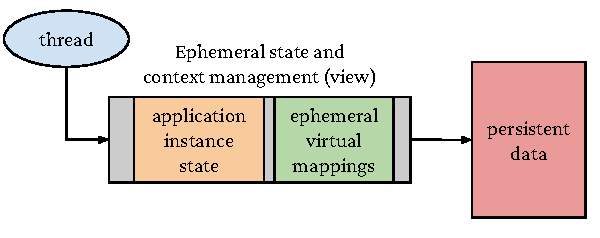
\includegraphics[width=\linewidth]{fig/view2}
    \caption[View objects in Twizzler]{View objects in \Twizzler. Views manage ephemeral constructs and state, giving threads
        the necessary context to execute and access persistent data.}
    \label{fig:view2}
\end{SCfigure}


By coalescing this ephemeral state
into an object, we make it possible for applications to manage it directly with minimal kernel
involvement. Avoiding the kernel is natural---all data access already does this in \Twizzler, so
adding a separate kernel API to manage this state would add complexity---and reduces the number of
system calls needed when mapping objects. Additionally, avoiding the kernel necessitates an
increased address space management responsibility for userspace. For example, executable loading
and mapping is largely handled without the kernel.

Applications can add objects to a view with the \texttt{view\_set} function. The caller specifies a
target object and a set of protections (see Chapter~\ref{ch:invariant}), and a slot in which to
map the object. However, applications rarely invoke this function directly---instead,
\texttt{libtwz} provides a higher-level API to allow applications to operate above the level of
manually mapping objects. The standard library also provides access to other utility functions for
views (such as querying state, creating new views, and copying views). These functions, by default,
operate on a thread's current view, but they optionally operate on any other view object\sidenote{Given appropriate
    permissions, of course.},
which allows \Twizzler to implement operations with semantics similar to \texttt{fork} and \texttt{execve}\sidenote{And
    introspection and debugging!}.

When threads add entries to a view object they need not inform the kernel---when
a fault occurs, the kernel will read the entry as needed. However, when \emph{changing} or
\emph{deleting} an entry, threads must inform the kernel so it can update existing page table entries.
We provide two system calls for views. The \texttt{become} system call allows a thread to
change to a new view, which might be used to execute a new program or jump across programs to, for
example, accomplish a protected task. \Twizzler's access control system prevents this from happening
arbitrarily. The second system call is \texttt{invalidate\_view}, which lets a thread inform the
kernel of changed or deleted entries.

View objects not only reduce kernel boundary crossings, but they also improve the resumability of
the system. After a power cycle, the OS now has information on which objects were mapped and where,
improving the ability of threads to pick up where they left off. Additionally, view objects
facilitate the sharing of address spaces between threads, since they can both synchronize on
modifying a given view object and need not duplicate information. Note that the particular contents
of a view object are system-specific. On virtual memory systems, one of their jobs is to manage
ephemeral virtual mappings, while on other architectures one of their jobs may be to manage, \eg, segment
tables. In all cases, views provide a mechanism for managing ephemeral state while
providing enough context for threads to execute.

\subsection{Threads}

\Twizzler provides a set of threading primitives for applications. Threads in \Twizzler are always
attached to a view and one or more security contexts. Threads may communicate with each other using
shared memory and can signal each other with a system call.
Since everything in \Twizzler is an object, each thread has a state object associated
with it. Signals can be raised assuming the raiser has appropriate permissions on the state object,
and the state object contains information about the thread.

A key primitive in \Twizzler is the \texttt{thread-sync} system call. This call operates similar to
\texttt{futex(2)} on Linux, except that it supports waiting on and waking up a number of different
words of memory simultaneously. Multi-word thread-sync is necessary to support
\texttt{select(2)}-like or \texttt{poll(2)}-like operations in a system where all data access is
done with memory semantics. \Twizzler's standard library exposes an API for event handling that uses
multi-word thread-sync, where objects may expose a set of ``events'' that can be triggered and waited for. This is
used in numerous places to implement event handling for multiple communications streams implemented
in objects.

\subsection{Program Instancing}

Programs can be loaded and run as ELF objects specifically linked for Twizzler. We provide a linker script that links
program data into virtual addresses that correspond to the first few view slots in an address space. This way an ELF
file can be loaded as a simple copy-from operation from the ELF object into several new objects (\eg, a \texttt{text},
\texttt{rodata}, and \texttt{data} object). Program components like thread-local storage, stack, and heap can also be
created out of objects. Finally, Twizzler supports a \texttt{fork}-like operation that copies a view object into a new
view, remapping and applying copy-on-write copy-from operations as needed.

\section{Security}
\label{sec:sec}


\Twizzler's focus on memory-based objects requires that we design the security model around
hardware-based enforcement, where the MMU checks
each access. This design is \emph{inevitable} in a data-centric OS, since the
kernel is not involved in every memory access. The kernel merely specifies the access rights when
mapping an object and then relies on the hardware to enforce those rights with a low overhead.

A key design choice we make is \emph{late-binding on security}. Applications
request access to an object with permissions that they desire;
if they access the object in only allowed ways (\eg, only reading a read-only
object), no fault occurs.
%This differs from current interfaces like \texttt{open} and \texttt{mmap}.
This is because when we map an object (via a view), the kernel is not immediately involved, and so
cannot check access rights for a particular access at the time the mapping is setup. Performing an access rights check on
time of first access does not make sense either, as it associates a specific access (that
might be allowed) with a permissions error. For example, if a program reads object $A$, and that program is
allowed to read $A$, it should be allowed to perform the read even if it requested read-write access
to the object.
This late-binding enables simpler programs that need not worry about
elevating access rights through remapping data objects. Programs can make progress without
knowing in advance the permissions of the objects they might access, thus enabling the reuse of the
OS's access control mechanism in applications, as we saw in the previous chapter.

Threads run in a security context~\cite{lwc,bittau:nsdi08,elhajj:asplos16}, which
contains a list of access rights for objects and allows the kernel to determine the access rights of
programs. Using these contexts, \Twizzler is able to provide
analogues to groups and owners in \unix while providing more fine-grained access control if
necessary. Unlike past exploration into security contexts, data-centric OSes offer an
advantage in simplicity. A security context abstraction in a \unix-like OS needs to
maintain access rights to a set of fundamentally different things, such as paths, virtual memory
locations, and system calls. Instead, \Twizzler's security contexts specify access rights to an object
via IDs instead of virtual addresses.
This also makes security contexts persistent, allowing us to use them as
the primary way we assign security roles to threads.


\subsection{Security Contexts and Page Tables}
\label{sec:secimpl}
Previously, we discussed how view objects allow applications to specify what objects they
want mapped in, and with what protections. These are merely \emph{requests}, however. Of course if
the thread does not have the appropriate \emph{permissions} the kernel will program the address
translation hardware appropriately. This presents a problem: since threads can attach to a number of
different security contexts, the number of different page-table structures that the kernel needs to
manage grows quickly.

\Twizzler uses Intel's Extended Page Table (EPT) technology\sidenote{Other architectures (and AMD) have similar systems, but
    \Twizzler does not support them yet.}, which is part of the virtualization
extensions. The EPT allows a virtual address to be translated by two separate page tables, and is
commonly used to virtualize the MMU in virtual machines. The first
level, using normal MMU page tables, translates a virtual address to an object-logical
address---typically with second-level address translation this is referred to as the
``guest-physical'' address---and the second-level translates this to a physical address.
We discussed this two-level scheme previously in Chapter~\ref{ch:global}, but here we can use the functionality to
gain security benefits.

Two-level address translation via the EPT enables \Twizzler to split protection \emph{requests}
and access control permissions. At the top-level, \Twizzler applies the requested protections from
the view maps without restriction, and programs the EPT to enforce access control derived from
the currently active security context. Splitting protection and access control is what allows applications to map
objects in for whatever access mode they would like without having to worry about first checking
permissions.
Furthermore, by separating out the permissions enforcement from ephemeral state and location
mapping, we reduce the number of page table structures the kernel needs to manage
from $O\left(n m\right)$ to $O\left(n + m\right)$, where $n$ is the number of views
and $m$ is the number of security contexts. Views and security contexts can also be switched out
independently from each other, which more closely fits the semantics of \Twizzler.

Two-level mapping also greatly simplifies the design of the kernel. Since mapping objects to physical memory
is done at the second level, page eviction is easy---the kernel can simply modify the shared page
tables stored per-object, which updates the translation for all views and contexts on the system after appropriate coherence. Moving objects between DRAM and \NVM is made easier
because objects reside in a given location within object-logical space regardless of where they are
mapped in virtual memory, so the kernel does not need to maintain back pointers to update page table
structures.


\subsection{Virtualization Hardware}
\Twizzler's use of virtualization hardware for normal operation is a limitation of existing
processors. Intel does not have a mechanism for using the EPT without switching on the entire
virtualization system and running in VMX-non-root mode. In practice, the additional
overhead from running with virtualization is negligible because we do not need all the protection of
a traditional virtual machine and so we can switch much of it off. Because \Twizzler's kernel is its own
guest, we can avoid much of the overhead introduced by VM exits necessary in lower-trust VM models.
For example, \Twizzler's kernel is allowed to modify the EPT structures itself, despite being
virtualized, and modern processors contain extensions that allow the guest to switch out EPTs itself
and handle EPT faults without triggering a VM exit.

This pairs nicely with using the IOMMU\sidenote{As much as the IOMMU is able to ``pair nicely'' with anything.} as well---since EPT structures on Intel can be reused in the
IOMMU, we can apply security contexts to drivers as well, making driver code less of a special case.
For example, \Twizzler provides a driver model for userspace drivers that allows driver code to
construct security contexts that explicitly map in only the necessary objects that a device might
need to access (\eg command queues, data objects, \emph{etc.}). As hardware devices grow in complexity and
increase their autonomy, treating them as additional computation resources and limiting access to
objects through mechanisms already in-place for normal applications allows simpler programming of
advanced hardware devices.





\iffalse
    \unedit {
        A \textit{capability} is, at its core, an unforgeable token which
        grants a particular set of rights on an object~\cite{Lampson1973,Landwehr1981,Gong:sigops89}. A
        given capability must be protected from tampering, accessible only to a process which is authorized
        to have it, and obtainable only through some secure mechanism. Many of the systems discussed above
        use capabilities, albeit in different forms. Some are secure because they are stored in-kernel and
        accessed via indirection (\unix file descriptors), while some are password-based, granting access
        when the kernel matches the provided password against an ACL. In most cases, however, these systems
        require secure capability information to be stored, protected, in kernel-only memory. This limits
        the power of these systems and requires significant kernel involvement whenever a security decision
        is made.  Instead, \emph{signed} capabilities can be used~\cite{tanenbaum:osr81}, which allow the
        kernel to verify the contents of a capability without needing to call out to a secure service or
        trust that it has not been modified.
        This approach has obvious benefits for distributed systems and for systems with long-life persistent
        data, but has not seen significant research as an operating systems security concept over the past
        few decades.
    }
\fi

\section{POSIX Compatibility}
\label{sec:legacy}

Twizzler provides a compatibility framework for POSIX applications. C applications link to a patched version of \texttt{musl}~\cite{musl}, a
C library written for Linux. We have modified \texttt{musl} to emit function calls to a library we wrote, called
\texttt{twix}, instead of directly issuing system calls. The calls into \texttt{twix} are then handled by emulating their
Linux system call behavior. For example, our implementation of \texttt{write(2)} allows us to create pseudo-terminal objects
that are shared between applications and a terminal emulator that is hooked up to the serial port. Thus applications
can call \texttt{printf} to get their messages out to wider society. Rust applications do not need as much of a compatibility layer, both because we can modify
Rust's standard library more easily, and because Rust is not as tied to POSIX as C is.

\subsection{Porting to Twizzler}

Porting in \Twizzler is straight-forward. We have a collection of tools that provide a
framework for compiling software using the \Twizzler toolchain against other ported software and
libraries. Since we have chosen \texttt{musl} as our standard C library, many applications work
already with minor changes. However, it is often the case that applications require
some small tweaks to get running---for example, configuration paths---an experience common for anyone who has ported software to a new
operating system\sidenote{You can't see it, but I am raising my glass to you, those who have shared in this experience.}.

To date, we have ported a number of tools one would expect to find on a \unix system, such as
\texttt{busybox} (providing numerous command-line utilities), \texttt{bash}, \texttt{vim},
\texttt{gcc}, \texttt{binutils}, and others. Many of these programs required little or no
modification. Of course, this means that they do not gain some of the benefits \Twizzler's model
provides, since they still operate on persistent data with a POSIX model, however our goal in
porting these tools was not to improve their performance, it was to provide a somewhat familiar
environment for users.

Perfect emulation of a Linux kernel is a huge effort, and it is not the primary goal of
our research. As a result, not all system calls are implemented and Linux features like
\texttt{procfs} are lacking. This means that some programs may require features that are not yet
implemented, and therefore require modifications to \texttt{twix} to run. However, as we continue to
port software, \texttt{twix}'s coverage of Linux features grows, making future porting easier. We
will continue to implement more support in \texttt{twix} for applications as needs arise. Note that
many applications (even complex applications like \texttt{gcc}) often boil down to reading and
writing files and managing processes, all of which is implemented.

\subsection{Twix System Call Overhead}

Our \unix emulation layer, \texttt{twix}, is meant to provide compatibility for legacy applications.
While we expect that applications will wish to take full advantage of \NVM and \Twizzler's
improvements in programmability and performance, we can still provide a small benefit
for applications that rely on \texttt{twix} to provide POSIX-like I/O. Access to \texttt{twix} is
done by \texttt{musl}, the C library we use, when it would normally perform a system call to a Linux
kernel. We replaced all instances of the \texttt{syscall} instruction in C and assembly code in
\texttt{musl} with a \texttt{call} instruction to an entry point in \texttt{twix}. This entry point,
despite being a function call, obeys the Linux system call ABI (\eg which registers hold
parameters). Thus while it has significantly less overhead than a full system call and context
switch, it does still have higher overhead than a normal function call since it must back up and
restore all registers.


\begin{SCtable}[b]
    \centering
    \caption[Emulated syscall latency]{Latency of selected \texttt{twix} system calls compared to Linux system calls.}
    \begin{minipage}{\linewidth}
        \centering
        \begin{tabular}{c | c | S[table-format=6.1]@{\,\,\( \pm \)\hspace{-7mm}} S[table-format=0.1]}
            \textbf{System Call} & \textbf{OS} & \multicolumn{2}{c}{\textbf{Average Latency (ns)}}       \\
            \hline
            \hline
            \texttt{getpid}      & Linux       & 98.7                                              & 2.3 \\
                                 & Twizzler    & 10.2                                              & 0.2 \\
            \hline
            \texttt{read}        & Linux       & 321.4                                             & 0.2 \\
                                 & Twizzler    & 55.4                                              & 0.2 \\
        \end{tabular}
    \end{minipage}
    \label{tbl:twix}
\end{SCtable}

Table~\ref{tbl:twix} shows the latency of some selected system calls on both Linux and \Twizzler
(implemented via \texttt{twix}). As expected, \texttt{getpid}'s overhead is small on both systems,
but on \Twizzler it is significantly lower. The difference, in this case, comes largely from the
kernel entry overhead. A small amount of additional overhead comes from
\texttt{twix} matching the Linux system call ABI and having to call its \texttt{getpid}
implementation through a lookup table.

We also measured the latency of a call to \texttt{read} for a file. We chose to do reads on cached
files for a small number of (already cached) bytes to avoid device transfer overhead. Performing a file read on
\Twizzler often amounts to a call to \texttt{memcpy}, so applications that perform large numbers of
small reads could see some benefit. In contrast, on Linux, the kernel needs to traverse internal
file structures, the page-cache, and possibly file system structures.
However, as we said, \texttt{twix} is intended for legacy
support, not performance, despite the lower system call overhead.
%As \texttt{read}
%lengths increase, we expect to see the system call overhead diminish relative to the cost of copying
%bytes into the buffer.

\begin{chconc}
    We now have an understanding of what addressing and pointers look like in Twizzler, and a basic idea of the
    operating system services Twizzler provides. One can write programs, multi-thread them, synchronize across
    threads via object sync words, access, create, copy, and
    delete objects, and use \unix compatibility for things like \texttt{printf}. But this still doesn't address issues
    of memory safety, types, and failure-atomicity. Join us in the next chapter where we will start diving into these
    scary topics.
\end{chconc}